% Einbinden von Variablen (Titel, Autor, usw.)
% Metainformationen zur Arbeit. 

% Titel des Dokuments
\newcommand{\titel}{Entwicklung eines Smart Home Systems mit Steuerung durch Android Apps}

% Zusätzlicher Untertitel
\newcommand{\untertitel}{Einen Untertitel gibt es auch noch}

% Autor
\newcommand{\autor}{Alexander \textsc{Hatzold} \& Patrick \textsc{Sudhaus}}

% Beide Autoren zusammen (nicht die von oben nehmen, da Text formatiert), Komma separiert
\newcommand{\pdfautor}{Hatzold, Sudhaus}

% Beide Autoren zusammen (nicht die von oben nehmen, da Text formatiert), und separiert
\newcommand{\footautor}{Alexander Hatzold, Patrick Sudhaus}

\newcommand{\matrikelnummer}{158105, 158116}

\newcommand{\kurs}{}

\newcommand{\bereich}{Angewandte Informatik}

% Betreuer der Arbeit
\newcommand{\betreuera}{Prof. Dr. Ulf \textsc{Schemmert}}
\newcommand{\betreuerb}{}

\newcommand{\abgabedatum}{\today}

% Art der Arbeit (z.B. Studienarbeit)
\newcommand{\art}{\Large Technische Dokumentation}

% Fachbereich der Arbeit
\newcommand{\fachbereich}{Angewandte Informatik}

% Jahr der Arbeit
\newcommand{\jahr}{2018}

% Universität
\newcommand{\uni}{\textsc{\LARGE{Hochschule fuer Telekommunikation Leipzig}}}

% Arbeitgeber
\newcommand{\job}{\textsc{\LARGE{T-Systems International GmbH}}}

% Tags, für das PDF Dokument
\newcommand{\tags}{smarthome, led, nodemcu, arduino}

\newcommand{\glossar}{\newglossaryentry{ecm}{
	type=\acronymtype,
	name={ECM},
	description={Enterprise Content Management},
	first={Enterprise Content Management (ECM)},
	%see=[Glossar:]{ecmg}
}

%\newglossaryentry{ecmg}{
%	name={Enterprise Content Management System},
%	description={Enterprise Content Management Systeme dienen zur Erfassung, Verwaltung, Speicherung, Bewahrung und Ausgabe von Informationen}
%}


\newglossaryentry{xml}{
	type=\acronymtype,
	name={XML},
	description={eXtensible Markup Language},
	%see=[Glossar:]{xmlg}
}

%\newglossaryentry{xmlg}{
%	name={eXtensible Markup Language},
%	description={XMl ist eine vom W3C verabschiedete Auszeichnungssprache, mit der sich hierarchische Strukturen darstellen lassen. Die erstellten Dokumente sind vom Menschen lesbar und bieten ein Format, welches mit dem Computer verarbeitet werden kann.}
%}

\newglossaryentry{Dokument}{
	name={Dokument},
	plural={Dokumente},
	description={Laut der ImageMaster Terminologie besitzt ein Dokument eine spezifische ID und ist einem \gls{Dokumententyp} zugeordnet. Einem Dokument können mehrere Dateien zugeordnet werden}
}

\newglossaryentry{Dokumententyp}{
	name={Dokumententyp},
	plural={Dokumententypen},
	description={Ein Dokumententyp beinhaltet Attribute nach denen später gesucht werden kann. \textbf{Beispiel:} Eine Rechnung mit den Attributen Rechnungsdatum, Kundennummer und Rechnungsbetrag.}
}

\newglossaryentry{AIIM}{
	type=\acronymtype,
	name={AIIM},
	description={Association for Information and Image Management},
	first={\textit{Association for Information and Image Management} (AIIM)},
	%see=[Glossar:]{aiimg}
}

\newglossaryentry{aiimg}{
	name={Association for Information and Image Management},
	first={\textit{Association for Information and Image Management} (AIIM)},
	description={Der AIIM ist eine Organisation, welche sich das Ziel gesetzt hat, Benutzern zu helfen die Herausforderungen in der Dokumentenverwaltung zu verstehen.}
}

\newglossaryentry{Revisionssicherheit}{
	name={Revisionssicherheit},
	description={Eine Revisionssichere Archivierung von Dokumenten bedeutet, dass diese nicht mit neueren Versionen überschrieben werden. Möchte man eine aktualisierte Version eines Dokuments abspeichern, bleiben alle älteren Versionen erhalten und es kann weiterhin auf sie zugegriffen werden.}
}

\newglossaryentry{Java EE}{
	type=\acronymtype,
	name={Java EE},
	description={Java Enterprise Edition},
	first={\textit{Java Enterprise Edition} (Java EE)},
%see=[Glossar:]{javaee}
}

\newglossaryentry{javaee}{
	name={Java EE},
	description={Java Enterprise Edition ist eine Spezifikation für die Softwarearchitektur auf Java basierenter Anwendungen, insbesondere Web-Anwendungen. Die Spezifikation definiert Dienste und Softwarekomponenten, sowie deren Schnittstellen über die sie mit anderen Komponenten kommunizieren können. Anhand dieser Spezifikation lassen sich mehrschichtige Anwendungen aufbauen und auf mehrere Systeme vertielen.}
}

\newglossaryentry{SOAP} {
	type=\acronymtype,
	name={SOAP},
	description={Simple Object Access Protocol},
	first={\textit{Simple Object Access Protocol} (SOAP)},
	%see=[Glossar:]{soapg}
}

\newglossaryentry{soapg} {
	name={SOAP},
	description={SOAP ist ein Netzwerkprotokoll mit dem Information zwischen verschiedenen Computersystemen ausgetauscht und Remote Procedure Calls durchgeführt werden können. Dabei stützt sich SOAP bei den Nachrichten auf das XML Format. [siehe \url{http://.w3schools.com/soap/}]}
}

\newglossaryentry{WSDL} {
	type=\acronymtype,
	name={WSDL},
	description={Web Service Description Language},
	first={\textit{Web Service Description Language} (WSDL)},
	%see=[Glossar:]{wsdlg}
}

\newglossaryentry{wsdlg} {
	name={WSDL},
	description={WSDL ist eine Beschreibungssprache für Webservices. Sie enthält alle Methoden, die ein Webservice bereitstellt und zeigt wie diese zu implementieren sind.}
}

\newglossaryentry{Metadaten} {
	name={Metadaten},
	description={Metadaten sind beschreibende Daten. Sie enthalten Informationen und beschreibungen zu anderen Daten. Metadaten zum Datum ``Name'' sind zum Beispiel Informationen was dieses Datum aussagt und wie es zu verwenden ist.}
}

\newglossaryentry{jms} {
	type=\acronymtype,
	name={JMS},
	first={\textit{Java Message Service} (JMS)},
	description={Java Message Service},
	%see=[Glossar:]{jmsg}
}

\newglossaryentry{jmsg} {
	name={JMS},
	description={\textbf{Java Message Service} ist eine Programmierschnitstelle zum Senden und Empfangen von Nachrichten aus einem Client heraus. Ziel dabei ist es, lose gekoppelte asynchrone Kommunikation zwischen den Komponenten einer verteilten ANwendung zu ermöglichen.}
}

\newglossaryentry{simple}{
	name={Simple Framework},
	description={\href{http://simple.sourceforge.net/home.php}{Simple Framework} ist ein API in Java, mit der man eine \gls{xml}-Datenbindung erreichen kann. Es ist damit möglich, Daten aus einer XML-Schema-Instanz heraus automatisch an Java-Klassen zu binden, und diese Java-Klassen aus einem XML-Schema heraus zu generieren \cite{wiki:jaxb}. Damit können XML-Dokumente eingelesen, bearbeitet und wieder geschrieben werden. }
}

\newglossaryentry{https}{
	type=\acronymtype,
	name={HTTP/S},
	first={\textit{HyperText Transfer Protocol (Secure)} (HTTPS)},
	description={HyperText Transfer Protocol (Secure)},
	%see=[Glossar:]{httpsg}
}

\newglossaryentry{httpsg}{
	name={HyperText Transfer Protocol Secure},
	description={HyperText Transfer Protocol Secure ist ein  ein Kommunikationsprotokoll im World Wide Web, um Daten abhörsicher zu übertragen. Es stellt eine Transportverschlüsselung dar. \citation{https}}
}

\newglossaryentry{API}{
	type=\acronymtype,
	name={API},
	first={\textit{Application Programming Interface} (API)},
	description={Application Programming Interface},
	%see=[Glossar:]{APIg}
}

\newglossaryentry{APIg}{
	name={Application Programming Interface},
	description={Eine API ist eine Programmierschnittstelle, mit deren Hilfe es möglich ist, anderen Programmen eine Anbindung an das jeweilige System herzustellen. Hierzu existieren im Regelfall umfangreiche Dokumentationen für den Programmierer.}
}

\newglossaryentry{REST}{
	type=\acronymtype,
	name={REST},
	first={\textit{Representational State Transfer} (REST)},
	description={Representational State Transfer},
}



\newglossaryentry{URI}{
	type=\acronymtype,
	name={URI},
	first={\textit{Uniform Resource Identifier} (URI)},
	description={Uniform Resource Identifier},
}

\newglossaryentry{IMAP}{
	type=\acronymtype,
	name={IMAP},
	description={Internet Message Access Protocol},
	first={\textit{Internet Message Access Protocol} (IMAP)},
	%dsee=[Glossar:]{imap}
}

\newglossaryentry{POP}{
	type=\acronymtype,
	name={POP},
	description={Post Office Protocol},
	first={\textit{Post Office Protocol} (POP)},
	%dsee=[Glossar:]{pop}
}

\newglossaryentry{SMTP}{
	type=\acronymtype,
	name={SMTP},
	description={Simple Mail Transfer Protocol},
	first={\textit{Simple Mail Transfer Protocol} (SMTP)},
	%dsee=[Glossar:]{smtp}
}

\newglossaryentry{JAMES}{
	type=\acronymtype,
	name={JAMES},
	description={Java Apache Mail Enterprise Server},
	first={\textit{Java Apache Mail Enterprise Server} (Apache James)},
	%see=[Glossar:]{jamesg}
}

\newglossaryentry{jamesg}{
	name={Apache James},
	description={\gls{JAMES} ist ein Mailserver, der im Enterprise-Bereich eingesetzt wird. Er beruht dabei komplett auf der Programmiersprache Java, sodass die Plattformunabhängigkeit gewährleistet ist \cite{a:james}.}
}

\newglossaryentry{servlet}{
	name={Servlet},
	plural={Servlets},
	description={\gf{Servlets sind Java-Programme, die in einem besonders präparierten Java-Webserver ausgeführt werden.}\cite{rw:javainsel}} 
}
}

\documentclass[
	12pt,			% Schriftgröße
	DIV14,			% Standard
	ngerman,		% Sprache
	a4paper,		% Papierformat
	titlepage,		% Es wird eine Titelseite verwendet
%	twoside,		% Zweiseitiges Layout
%	BCOR=10mm,		% 10mm für Bindung berücksichtigen
	parskip=half,	% Halber Zeilenabstand
%	lists=totoc,		% Verzeichnisse im Inhaltsverzeichnis aufführen
	bibliography=totoc,		% Literaturverzeichnis im Inhaltsverzeichnis aufführen
%	idx=totoc,		% Index im Inhaltsverzeichnis aufführen
	final			% Abschließend
]{scrreprt}

% Einbinden aller Pakete
% F�r umbr�che
\usepackage[ngerman]{babel}

% Umlaute
\usepackage[utf8]{inputenc}
\usepackage[T1]{fontenc}
\usepackage{lmodern}

% Es k�nnen Tabellen erstellt werden, die eine feste Gesamtbreite haben
\usepackage{tabularx}
\usepackage{tabulary}

\usepackage{layout}

% Euro-Zeichen etc
\usepackage{textcomp}

% Grafiken
\usepackage[dvips,final]{graphicx}
% Dort liegen die Bilder des Dokuments
\graphicspath{{images/}}
% Zum Umflie�en von Bildern
\usepackage{floatflt}

\usepackage[numbers, square]{natbib}

% Caption �ber der Tabelle / dem Code
\usepackage{floatrow}
\usepackage{tabu}

\usepackage{longtable}

\usepackage{dirtree}

\usepackage{fancyvrb}

%Definition der Farben in includes/colors
\usepackage[usenames,dvipsnames,table]{xcolor} 

% Package zum formatieren von Code
%\usepackage[chapter]{minted}

% Zum Einbinden von Programmcode
\usepackage{listings}

% Einstellungen f�r Listings, kann wahrscheinlich weg???
\lstset{%
    float=hbp,%
    basicstyle=\texttt\small, %
    identifierstyle=\color{colIdentifier}, %
    keywordstyle=\color{colKeys}, %
    stringstyle=\color{colString}, %
    commentstyle=\color{colComments}, %
    columns=flexible, %
    tabsize=2, %
    frame=single, %
    extendedchars=true, %
    showspaces=false, %
    showstringspaces=false, %
    numbers=left, %
    numberstyle=\tiny, %
    breaklines=true, %
    backgroundcolor=\color{hellgelb}, %
    breakautoindent=true, %
%    captionpos=b%
}


% Abk�rzungen
\usepackage{acronym}

% F�r Index-Ausgabe; \printindex
\usepackage{makeidx}

% Einfache Definition der Zeilenabst�nde und Seitenr�nder etc.
\usepackage{setspace}
\usepackage[top=3cm, bottom=3.5cm]{geometry}

\usepackage[
	automark,		% Kapitelangaben in Kopfzeile automatisch erstellen
	headsepline,	% Trennlinie unter Kopfzeile
	ilines			% Trennlinie linksb�ndig ausrichten
]{scrlayer-scrpage}

% PDF-Optionen
\usepackage[
	bookmarks,
	bookmarksopen=true,
	pdftitle={\titel},
	pdfauthor={\pdfautor},
	pdfcreator={\pdfautor},
	pdfsubject={\titel},
	pdfkeywords={\tags},
	colorlinks=true,
	linkcolor=magenta, 		% einfache interne Verkn�pfungen
	%linkcolor=black,
	anchorcolor=green,		% Ankertext
	citecolor=dhbwred,			% Verweise auf Literaturverzeichniseintr�ge im Text
	%citecolor=black,
	filecolor=magenta, 		% Lokale Dateien
	%filecolor=black,
	menucolor=compred,
	%menucolor=black, 		% Acrobat-Men�punkte
	urlcolor=cyan,
	%urlcolor=black, 
	plainpages=false,		% zur korrekten Erstellung der Bookmarks
	pdfpagelabels,			% zur korrekten Erstellung der Bookmarks
	hypertexnames=false,	% zur korrekten Erstellung der Bookmarks
	linktocpage 			% Seitenzahlen anstatt Text im Inhaltsverzeichnis verlinken
]{hyperref}

% URL 
\usepackage{url}

% G�nsef��chen mit \enquote{text}
\usepackage{csquotes}

% F�r die Chapter Formatierung 
\usepackage{blindtext, color}

% Zum fortlaufenden Durchnummerieren der Fu�noten
%\usepackage{chngcntr}

% Eigene Caption Definition mit Style
\usepackage{caption}

% Eigene Subcaption Definition mit Style
\usepackage{subcaption}

% Chapterstyle
\usepackage[explicit]{titlesec}
\usepackage{lmodern}

\usepackage{todonotes}

%https://en.wikibooks.org/wiki/LaTeX/Glossary
\usepackage[	 
	toc,   
	%xindy,
	%nomain,
	nopostdot,
	%Zahl, die Kapitel anzeigt, in dem das Wort gebraucht wurde
	nonumberlist,
	seeautonumberlist,
	acronym]      
{glossaries}

\usepackage{tikz}
\def\checkmark{\tikz\fill[scale=0.4](0,.35) -- (.25,0) -- (1,.7) -- (.25,.15) -- cycle;} 

\makeglossaries

\makeindex

% Farben und einige eigene Definitionen
\definecolor{hellgelb}{rgb}{1,1,0.9}
\definecolor{colKeys}{rgb}{0,0,1}
\definecolor{colIdentifier}{rgb}{0,0,0}
\definecolor{colComments}{rgb}{1,0,0}
\definecolor{colString}{rgb}{0,0.5,0}
\definecolor{darkcyan}{RGB}{59, 188, 211}
\definecolor{compred}{RGB}{211, 82, 59}
\definecolor{dhbwred}{RGB}{226, 0, 26}
\colorlet{lightdhbwred}{dhbwred!5}
\definecolor{dhbwgrey}{RGB}{93, 105, 113}
\colorlet{lightdhbwgrey}{dhbwgrey!20}
\definecolor{lightgrey}{RGB}{224, 224, 224}

\definecolor{magenta}{RGB}{226,0,116}

% Einbinden des Seitenlayouts
% Zeilenabstand auf 1,5
\onehalfspacing

% Nummerierungstiefe
\setcounter{secnumdepth}{2}
\setcounter{tocdepth}{2}

% Kopf- und Fußzeile
\pagestyle{scrheadings}

% Kopf- und Fußzeile auch auf Kapitelanfangsseiten
\renewcommand*{\chapterpagestyle}{scrheadings}

%Verzeichnis für Programmcode
%\renewcommand{\listoflistingscaption}{Quellcodeverzeichnis}
%\renewcommand{\listingscaption}{Code}

% Schriftform der Kopfzeile
\renewcommand{\headfont}{\normalfont}

% Damit Programmcode auch über mehrere Seiten hinweg eingefügt werden kann
%\newenvironment{code}{\captionsetup{type=listing}}{}

% Schusterjungen und Hurenkinder vermeiden
\clubpenalty = 10000 %
\widowpenalty = 10000 
\displaywidowpenalty = 10000

% Table
%\taburulecolor{dhbwred!60}
%\rowcolors{1}{}{lightdhbwred}

% Größe der Kapitelnummer
\newlength\chapnumb
\setlength\chapnumb{4cm}

% Neue Definition für Chapter
\titleformat{\chapter}[block]
{\color{magenta}\normalfont\sffamily}{}{0pt}
{\parbox[b]{\chapnumb}{%
   \fontsize{120}{110}\selectfont\thechapter}%
  \parbox[b]{\dimexpr\textwidth-\chapnumb\relax}{%
    \raggedleft%
    \color{dhbwgrey}
    \hfill{\LARGE#1}\\
    \rule{\dimexpr\textwidth-\chapnumb\relax}{0.4pt}}}
    
% Neue Definition für Chapter ohne Nummerierung
\titleformat{name=\chapter,numberless}[block]
{\color{dhbwgrey}\normalfont\sffamily}{}{0pt}
{\parbox[b]{\chapnumb}{%
   \mbox{}}%
  \parbox[b]{\dimexpr\textwidth-\chapnumb\relax}{%
    \raggedleft%
    \hfill{\LARGE#1}\\
    \rule{\dimexpr\textwidth-\chapnumb\relax}{0.4pt}}}


% Neue Definition für Section
\titleformat{\section}
{\color{dhbwgrey}\normalfont\Large\bfseries}
{\color{magenta}\thesection}{1em}{#1}

% Neue Definition für Subsection
\titleformat{\subsection}
{\color{dhbwgrey}\normalfont\large\bfseries}
{\color{magenta}\thesubsection}{1em}{#1}

% Neue Definition für Subsubsection
\titleformat{\subsubsection}
{\color{dhbwgrey}\normalfont\normalsize\bfseries}
{\color{magenta}\thesubsubsection}{1em}{#1}

\titleformat{\paragraph}
{\color{dhbwgrey}\normalfont\normalsize\bfseries}
{}{0em}{\textit{#1}}

% Caption über der Tabelle / dem Code
%\floatsetup[listing]{style=Plaintop}
%\floatsetup[figure]{style=Plaintop}
%\floatsetup[table]{capposition=top}

% Kopfzeile
%Kopfzeile innen
\ihead{
	\textit{
		\textsc{\headmark}
	}
}
%Kopfzeile Mitte
\chead{}
% Kopfzeile außen - Logo
\ohead{
	
\includegraphics[scale=0.03]{../images/hftl_logo}\hspace{1.9cm}
}
\setlength{\headheight}{10mm} % Höhe der Kopfzeile

\setheadwidth[10pt]{textwithmarginpar} % Kopfzeile über den Text hinaus verarbeiten
\setheadsepline[text]{0.4pt} % Trennlinie unter Kopfzeile

\ifoot {
	\textit{\footautor} %Name des Kurses
}
\cfoot{}
\ofoot{
	\pagemark
}
\setfootsepline[text]{0.4pt} % Trennlinie über Fußzeile

% Neue Caption Definition
%\DeclareCaptionFont{white}{\color{dhbwgrey}}
%\DeclareCaptionFormat{}{\colorbox{lightdhbwgrey}{\parbox{\textwidth}{#1 #2#3}}}
%\captionsetup{format=listing,labelfont=white,textfont=white}

% Neue Subcaption Definition
%\DeclareCaptionFont{normal}{\color{dhbwgrey}}
%\DeclareCaptionFormat{subfig}{\parbox{\textwidth}{#1 #2#3}}
%\captionsetup[sub]{format=subfig, labelfont=normal, textfont=normal}

\definecolor{quotationcolour}{HTML}{F0F0F0}
\definecolor{quotationmarkcolour}{HTML}{1F3F81}

% Quotation
% Massively humongous opening quotation mark.
\newcommand{\hugequote}{%
  \fontsize{42}{48}\selectfont \color{magenta} \textbf{``}
  \vskip -.5em
}

% Beautify quotations.
\newcommand{\epigraph}[2]{%
  \begin{center}
  \colorbox{lightdhbwred}{%
    \parbox{.9\textwidth}{%
    	\hrule \vskip 1em {\hugequote} \vskip -.5em
    	\parindent 2.2em
    	#1\begin{flushright}\textsc{#2}\end{flushright}
    	\hrule
    }
  }
  \end{center}
  \bigskip
}

\renewcommand{\glsnamefont}[1]{\textcolor{dhbwgrey}{#1}}

% Neue Commands
% to-dos 
\newcommand{\td}[1]{\textbf{TODO: #1}}

% Zitierhilfe
\newcommand{\vgl}[2]{(vgl. \cite{#1}, S. #2)}
\newcommand{\vgltwo}[4]{(vgl. \cite{#1}, S. #2 und \cite{#3}, S. #4)}
\newcommand{\vgld}[2]{(\cite{#1}, S. #2)}

% Fachbegriffe in italics
\newcommand{\fb}[1]{\textit{#1}}

% Gänsefüßchen
\newcommand{\gf}[1]{\glqq{}#1\grqq{}}

% Abkürzungen
\newcommand{\ua}{\mbox{u.\,a.\ }}
\newcommand{\zb}{\mbox{z.\,B.\ }}
\newcommand{\bs}{$\backslash$}

\newcommand{\vip}[1]{\textsc{#1}}




% Abkürzungsverzeichnis
\newglossaryentry{ecm}{
	type=\acronymtype,
	name={ECM},
	description={Enterprise Content Management},
	first={Enterprise Content Management (ECM)},
	%see=[Glossar:]{ecmg}
}

%\newglossaryentry{ecmg}{
%	name={Enterprise Content Management System},
%	description={Enterprise Content Management Systeme dienen zur Erfassung, Verwaltung, Speicherung, Bewahrung und Ausgabe von Informationen}
%}


\newglossaryentry{xml}{
	type=\acronymtype,
	name={XML},
	description={eXtensible Markup Language},
	%see=[Glossar:]{xmlg}
}

%\newglossaryentry{xmlg}{
%	name={eXtensible Markup Language},
%	description={XMl ist eine vom W3C verabschiedete Auszeichnungssprache, mit der sich hierarchische Strukturen darstellen lassen. Die erstellten Dokumente sind vom Menschen lesbar und bieten ein Format, welches mit dem Computer verarbeitet werden kann.}
%}

\newglossaryentry{Dokument}{
	name={Dokument},
	plural={Dokumente},
	description={Laut der ImageMaster Terminologie besitzt ein Dokument eine spezifische ID und ist einem \gls{Dokumententyp} zugeordnet. Einem Dokument können mehrere Dateien zugeordnet werden}
}

\newglossaryentry{Dokumententyp}{
	name={Dokumententyp},
	plural={Dokumententypen},
	description={Ein Dokumententyp beinhaltet Attribute nach denen später gesucht werden kann. \textbf{Beispiel:} Eine Rechnung mit den Attributen Rechnungsdatum, Kundennummer und Rechnungsbetrag.}
}

\newglossaryentry{AIIM}{
	type=\acronymtype,
	name={AIIM},
	description={Association for Information and Image Management},
	first={\textit{Association for Information and Image Management} (AIIM)},
	%see=[Glossar:]{aiimg}
}

\newglossaryentry{aiimg}{
	name={Association for Information and Image Management},
	first={\textit{Association for Information and Image Management} (AIIM)},
	description={Der AIIM ist eine Organisation, welche sich das Ziel gesetzt hat, Benutzern zu helfen die Herausforderungen in der Dokumentenverwaltung zu verstehen.}
}

\newglossaryentry{Revisionssicherheit}{
	name={Revisionssicherheit},
	description={Eine Revisionssichere Archivierung von Dokumenten bedeutet, dass diese nicht mit neueren Versionen überschrieben werden. Möchte man eine aktualisierte Version eines Dokuments abspeichern, bleiben alle älteren Versionen erhalten und es kann weiterhin auf sie zugegriffen werden.}
}

\newglossaryentry{Java EE}{
	type=\acronymtype,
	name={Java EE},
	description={Java Enterprise Edition},
	first={\textit{Java Enterprise Edition} (Java EE)},
%see=[Glossar:]{javaee}
}

\newglossaryentry{javaee}{
	name={Java EE},
	description={Java Enterprise Edition ist eine Spezifikation für die Softwarearchitektur auf Java basierenter Anwendungen, insbesondere Web-Anwendungen. Die Spezifikation definiert Dienste und Softwarekomponenten, sowie deren Schnittstellen über die sie mit anderen Komponenten kommunizieren können. Anhand dieser Spezifikation lassen sich mehrschichtige Anwendungen aufbauen und auf mehrere Systeme vertielen.}
}

\newglossaryentry{SOAP} {
	type=\acronymtype,
	name={SOAP},
	description={Simple Object Access Protocol},
	first={\textit{Simple Object Access Protocol} (SOAP)},
	%see=[Glossar:]{soapg}
}

\newglossaryentry{soapg} {
	name={SOAP},
	description={SOAP ist ein Netzwerkprotokoll mit dem Information zwischen verschiedenen Computersystemen ausgetauscht und Remote Procedure Calls durchgeführt werden können. Dabei stützt sich SOAP bei den Nachrichten auf das XML Format. [siehe \url{http://.w3schools.com/soap/}]}
}

\newglossaryentry{WSDL} {
	type=\acronymtype,
	name={WSDL},
	description={Web Service Description Language},
	first={\textit{Web Service Description Language} (WSDL)},
	%see=[Glossar:]{wsdlg}
}

\newglossaryentry{wsdlg} {
	name={WSDL},
	description={WSDL ist eine Beschreibungssprache für Webservices. Sie enthält alle Methoden, die ein Webservice bereitstellt und zeigt wie diese zu implementieren sind.}
}

\newglossaryentry{Metadaten} {
	name={Metadaten},
	description={Metadaten sind beschreibende Daten. Sie enthalten Informationen und beschreibungen zu anderen Daten. Metadaten zum Datum ``Name'' sind zum Beispiel Informationen was dieses Datum aussagt und wie es zu verwenden ist.}
}

\newglossaryentry{jms} {
	type=\acronymtype,
	name={JMS},
	first={\textit{Java Message Service} (JMS)},
	description={Java Message Service},
	%see=[Glossar:]{jmsg}
}

\newglossaryentry{jmsg} {
	name={JMS},
	description={\textbf{Java Message Service} ist eine Programmierschnitstelle zum Senden und Empfangen von Nachrichten aus einem Client heraus. Ziel dabei ist es, lose gekoppelte asynchrone Kommunikation zwischen den Komponenten einer verteilten ANwendung zu ermöglichen.}
}

\newglossaryentry{simple}{
	name={Simple Framework},
	description={\href{http://simple.sourceforge.net/home.php}{Simple Framework} ist ein API in Java, mit der man eine \gls{xml}-Datenbindung erreichen kann. Es ist damit möglich, Daten aus einer XML-Schema-Instanz heraus automatisch an Java-Klassen zu binden, und diese Java-Klassen aus einem XML-Schema heraus zu generieren \cite{wiki:jaxb}. Damit können XML-Dokumente eingelesen, bearbeitet und wieder geschrieben werden. }
}

\newglossaryentry{https}{
	type=\acronymtype,
	name={HTTP/S},
	first={\textit{HyperText Transfer Protocol (Secure)} (HTTPS)},
	description={HyperText Transfer Protocol (Secure)},
	%see=[Glossar:]{httpsg}
}

\newglossaryentry{httpsg}{
	name={HyperText Transfer Protocol Secure},
	description={HyperText Transfer Protocol Secure ist ein  ein Kommunikationsprotokoll im World Wide Web, um Daten abhörsicher zu übertragen. Es stellt eine Transportverschlüsselung dar. \citation{https}}
}

\newglossaryentry{API}{
	type=\acronymtype,
	name={API},
	first={\textit{Application Programming Interface} (API)},
	description={Application Programming Interface},
	%see=[Glossar:]{APIg}
}

\newglossaryentry{APIg}{
	name={Application Programming Interface},
	description={Eine API ist eine Programmierschnittstelle, mit deren Hilfe es möglich ist, anderen Programmen eine Anbindung an das jeweilige System herzustellen. Hierzu existieren im Regelfall umfangreiche Dokumentationen für den Programmierer.}
}

\newglossaryentry{REST}{
	type=\acronymtype,
	name={REST},
	first={\textit{Representational State Transfer} (REST)},
	description={Representational State Transfer},
}



\newglossaryentry{URI}{
	type=\acronymtype,
	name={URI},
	first={\textit{Uniform Resource Identifier} (URI)},
	description={Uniform Resource Identifier},
}

\newglossaryentry{IMAP}{
	type=\acronymtype,
	name={IMAP},
	description={Internet Message Access Protocol},
	first={\textit{Internet Message Access Protocol} (IMAP)},
	%dsee=[Glossar:]{imap}
}

\newglossaryentry{POP}{
	type=\acronymtype,
	name={POP},
	description={Post Office Protocol},
	first={\textit{Post Office Protocol} (POP)},
	%dsee=[Glossar:]{pop}
}

\newglossaryentry{SMTP}{
	type=\acronymtype,
	name={SMTP},
	description={Simple Mail Transfer Protocol},
	first={\textit{Simple Mail Transfer Protocol} (SMTP)},
	%dsee=[Glossar:]{smtp}
}

\newglossaryentry{JAMES}{
	type=\acronymtype,
	name={JAMES},
	description={Java Apache Mail Enterprise Server},
	first={\textit{Java Apache Mail Enterprise Server} (Apache James)},
	%see=[Glossar:]{jamesg}
}

\newglossaryentry{jamesg}{
	name={Apache James},
	description={\gls{JAMES} ist ein Mailserver, der im Enterprise-Bereich eingesetzt wird. Er beruht dabei komplett auf der Programmiersprache Java, sodass die Plattformunabhängigkeit gewährleistet ist \cite{a:james}.}
}

\newglossaryentry{servlet}{
	name={Servlet},
	plural={Servlets},
	description={\gf{Servlets sind Java-Programme, die in einem besonders präparierten Java-Webserver ausgeführt werden.}\cite{rw:javainsel}} 
}


\begin{document}

		\thispagestyle{plain}

\begin{titlepage} 
	\begin{center}
		%\includegraphics[width=0.55\textwidth]{dhbw_logo_m}\\[1cm]
		\uni
		\\[1cm]
		
\includegraphics[scale=0.075]{../images/hftl_logo} \\
		[0.5cm]
		\art
		\\[0.7cm]
		\hrule
		\vspace{0,5cm}
		{\huge \textsc{\titel}} % Titel
		\\[0,9cm] 
		\hrule
		\vspace{1,5cm}
		%\begin{minipage}{0.4\textwidth}
			%\begin{flushleft} 
				\large \emph{Autor:}\\
				\autor \\
				\vspace{\baselineskip} %Leerzeile damit der Name auf der gleichen höhe ist wie der erste Autor
			%\end{flushleft} 
		%\end{minipage}
		%\begin{minipage}{0.4\textwidth} 
			%\begin{flushright}
				\large \emph{Betreuer:} \\ 
				\betreuera \\ 
				\betreuerb
			%\end{flushright} 
		%\end{minipage} 
		\vfill % Bottom ofthe page 
		{\large \today} 
	\end{center}
\end{titlepage}
\thispagestyle{empty}
\cleardoublepage

		\thispagestyle{plain}

\begin{titlepage}
	\begin{center}
		Diese Arbeit wurde vorgelegt von\\
		{\Large\footautor}\\[8ex]
		\begin{tabular}{rl}
			Hochschule: &\quad Hochschule für Telekommunikation Leipzig\\[1.2ex]
			Matrikelnummer: &\quad \matrikelnummer\\[1.2ex]
			%Kurs:  & \quad \kurs\\[1.2ex]
			Studienbereich: & \quad Angewandte Informatik\\[4ex]
			Betreuer: & \quad Prof. Dr. Ulf Schemmert\\[1.2ex]
			%Abgabedatum:  & \quad \abgabedatum\\[12ex]
		\end{tabular}
	
	
		\vspace*{\fill}
		\copyright\ \jahr\\[0.5ex]
		
		\singlespacing
		\small
		\noindent Dieses Werk einschließlich seiner Teile ist \textbf{urheberrechtlich geschützt}. Jede Verwertung außerhalb der engen Grenzen des Urheberrechtgesetzes ist ohne Zustimmung des Autors unzulässig und strafbar. Das gilt insbesondere für Vervielfältigungen, Übersetzungen, Mikroverfilmungen sowie die Einspeicherung und Verarbeitung in elektronischen Systemen.
	\end{center}
\end{titlepage}


		
		% Römische nummerierung
		\pagenumbering{Roman}
		
			% Ehrenwörtliche Erklärung
			%\input{../chapters/erklaerung}
			
			%\input{../chapters/danksagungen}
			
			% Abstact
			%\input{../chapters/abstract}
			
			% Inhaltsverzeichnis
			\tableofcontents
			
			% Abbildungsverzeichnis
			%\listoffigures
			
			% Tabellenverzeichnis					
			%\listoftables					
			
			% CodeVerzeichnis
			%\listoflistings	
			
			% weiter in normalen arabischen Ziffern
			\clearpage
			
		\pagenumbering{arabic}
		
			\chapter{Einleitung}

Im Zuge der Digitalisierung werden alle Bereiche des täglichen Lebens auf neue, digitale Systeme umgestellt. So wird beispielsweise im Bereich des Wohnens auf Technologien gesetzt, die über das Internet steuerbar sind. Damit einhergehend wird oft der Begriff des Internet of Things (IoT) genannt, zu dem auch der Bereich Smart Home gezählt werden kann.\\
Diese Dokumentation beschäftigt sich mit dem Entwurf und der Umsetzung einer Smart Home- Architektur und der Implementierung zweier Apps, die für die Steuerung der Komponenten in diesem Netzwerk genutzt werden sollen. Die erste App soll eine LED-Lichterkette in verschiedenen Modi ansteuern können. Die zweite Anwendung soll eine Multitimer-App darstellen, die als wichtiger Helfer im Haushalt und insbesondere beim Kochen agiert. Dabei ist diese Timer-App ebensfalls an das Smart Home-Netzwerk angebunden und kann einzelne Komponenten des Smart Homes steuern. \\
Das Ergebnis dieser Arbeit ist ein prototypisch implementiertes Netzwerk, in das die beiden Apps eingepflegt werden und die IoT-Geräte angesteuert werden können.
			\chapter{Grundlagen}
Um die weiteren Betrachtungen nachvollziehen zu können, werden an dieser Stelle die nötigen Grundlagen dargestellt.

\section{Message-Broker und MQTT} \label{introMQTT}

\textit{Message-Broker} gehören zu den nachrichtenorientieren Middlewares und sind Server- Anwendungen, die Nachrichten empfangen und weiterleiten. Dabei kann eine Umwandlung des Protokolls des Senders in ein für den Empfänger verständliches Protokoll geschehen. \\
\textit{Message Queue Telemetry Transport (MQTT)} ist ein Publish/Subscribe Messaging Transport Protokoll, das von einem Message Broker verwendet werden kann. Es ist leichtgewichtig, einfach aufgebaut, einfach zu implementieren und steht zur freien Verfügung. Damit soll gewährleistet werden, dass es vor allem für IoT-Anwendungen und für Machine-to-Machine (M2M)-Anwendungen geeignet ist, da hier häufig eine geringe Netzwerkbandbreite zur Verfügung steht. Als zugrundeliegendes Protokoll wird TCP/IP verwendet. \\
Das Publish/Subscribe-Verfahren funktioniert folgendermaßen:
\begin{description}
	\item[Publisher] Dieser Teilnehmer ist die sendende Instanz im Netzwerk. Jede Nachricht wird einer bestimmten Kategorie, auch Topic genannt, zugeordnet. Der Sender weiß dabei nicht, wer die Nachricht empfangen wird.
	\item[Subscriber] Der Subscriber oder Empfänger empfängt alle Nachrichten, zu deren Topic er sich beim Message-Broker registriert hat. Dieser Teilnehmer hat keine Kenntnis über die Herkunft der Nachricht.
	\item[Broker] Diese Instanz ist der Vermittler zwischen Publisher und Subscriber. Er empfängt alle Nachrichten und stellt sie allen relevanten Empfänger zu. 
\end{description}
Bei der Verwendung von MQTT gibt es drei Stufen des Quality of Service (QoS):
\begin{enumerate}
	\item QoS Level 0: Dieses Level agiert nach dem Ansatz \gf{At most once}, d.h. jede Nachricht wird maximal einmal zugestellt und sollte dies fehlschlagen, erfolgt keine erneute Zustellung. Dementsprechend können Nachrichten verloren gehen.
	\item QoS Level 1: Die unter dem Ansatz \gf{At least once} bekannte Stufe stellt Nachrichten mindestens einmal zu, wobei mehrmalige Zustellung nicht ausgeschlossen ist.
	\item QoS Level 2: Der \gf{Exactly once}-Ansatz stellt jede Nachricht genau einmal zu.
\end{enumerate}
Die Spezifikation von MQTT Version 3.1.1 ist unter \cite{mqtt_spec} verfügbar.

\section{Digitale LEDs}
Digitale LEDs erlauben es mit nur einem Datenkanal mehrere LEDs unterschiedlich anzusteuern. Dies wird durch den Einsatz eines Chips für jede LED möglich, der nur die für ihn relevanten Daten extrahiert und anzeigt. Hierdurch ergibt sich nicht nur die Möglichkeit, manuell jede LED mit einer bestimmten Farbe anzusteuern, sondern auch Effekte wie Lauflicht oder Regenbogen sind umsetzbar.\\
Für dieses Projekt wurde sich für WS2812B 5050 SMD LEDs entschieden, da diese einfach über Libraries mit dem Mikrocontroller ansteuerbar und verhältnismäßig kostengünstig sind. Zum Ansteuern dieser LEDs kann die populäre Arduino Library \gf{Adafruit Neopixels} verwendet werden.

			\chapter{Anforderungen \& Planung}

\section{Aufbau der Infrastruktur \& Technische Details}

Die Applikationen werden für das Betriebssystem Android in der Programmiersprache Java entwickelt, wobei auf API-Level 21 (Android 5.0) zurückgegriffen wird. Android Studio stellt dabei die Entwicklungsumgebung der Wahl dar. \\
Als Protokoll zum Austausch der Nachrichten wird das MQTT-Protokoll verwendet. Die zugrundeliegende MQTT-Software heißt \textit{Mosquitto}. \\
Die zentrale Serverkomponente \gf{Home Manager}, die für bestimmte Funktionen (siehe Abschnitt \ref{home_manager}) genutzt wird, wird ebenfalls in der Programmiersprache Java geschrieben. Dabei wird zum persistenten Speichern von Informationen die auf MySQL basierende Datenbank MariaDB verwendet. \\
Die Mikrocontroller, die für die Steuerung der LED-Lichterketten verantwortlich sind, basieren auf dem ESP8266 CPU. Der verwendete NodeMCU V3 koppelt diese Architektur mit einem WLAN-Chip und 13 GPIO Pins, wodurch der Mikrocontroller Nachrichten empfangen kann und Informationen für die Lichtsteuerung über GPIO Pins ausgeben kann. Das Programm auf diesen wird mithilfe der Arduino IDE in der Programmiersprache C geschrieben. \\ 
Die Infrastruktur ist in Abbildung \ref{fig:architecture} dargestellt. Die Android-Geräte mit den entsprechenden Apps werden im Folgenden als \textit{Sender} bezeichnet, da sie überwiegend Befehle zum Message-Broker senden. Dieser wertet die Nachrichten aus und stellt die den entsprechenden Empfängern zu. Die Nachrichten werden über das jeweilige Topic identifiziert, d.h. jede LED besitzt ein eigenes Topic, sodass jede LED einzeln angesteuert werden kann. Dabei folgen die Topics dem Schema \textit{Kanal/Zimmer/Gerät/Funktion}, sodass auch mehrere LED Streifen in einem Raum angesprochen werden können. Die Nachricht selbst enthält die Information, wie die LEDs leuchten sollen. Die Nachrichten werden von dem im WLAN-Netzwerk angemeldeten Mikrocontroller empfangen und verarbeitet. Diese im Folgenden als \textit{Empfänger} bezeichneten Geräte führen die gewünschte Aktion aus, bspw. das Leuchten der LED Steifen in den gewünschten Farben. \\
Für die Notation der Nachrichten wurde sich für JSON entschieden. 

\subsubsection*{Server-Komponente \textit{Home Manager}}
Die Nachricht wird außerdem noch vom sog. \textit{Home Manager} empfangen, der für sich relevante Nachrichten herausfiltert und verarbeitet. Zu seinen Funktionalitäten gehört die Umsetzung einer Timer-Funktion. In einer der beiden Apps soll eine Funktion eingebaut werden, um Timer einzustellen, d.h. dass zu bestimmten Uhrzeiten bestimmte LEDs automatisch angesteuert werden. So kann erreicht werden, dass man bspw. durch Hellwerden am Morgen geweckt wird oder abends das Licht bereits angeschaltet ist, wenn man nach Hause kommt. Dies soll durch Eintragungen der Zeitpunkte in die Datenbank MariaDB geschehen, welche in bestimmten Intervallen gelesen wird und die LEDs durch die HomeManager-Komponente aktiviert werden. Aufgrund der Komplexität und den Rahmenbedingungen dieser Arbeit im Rahmen des Moduls \gf{Mobile Applikationen} ist diese Funktion allerdings optional.


\begin{figure}
	\centering
	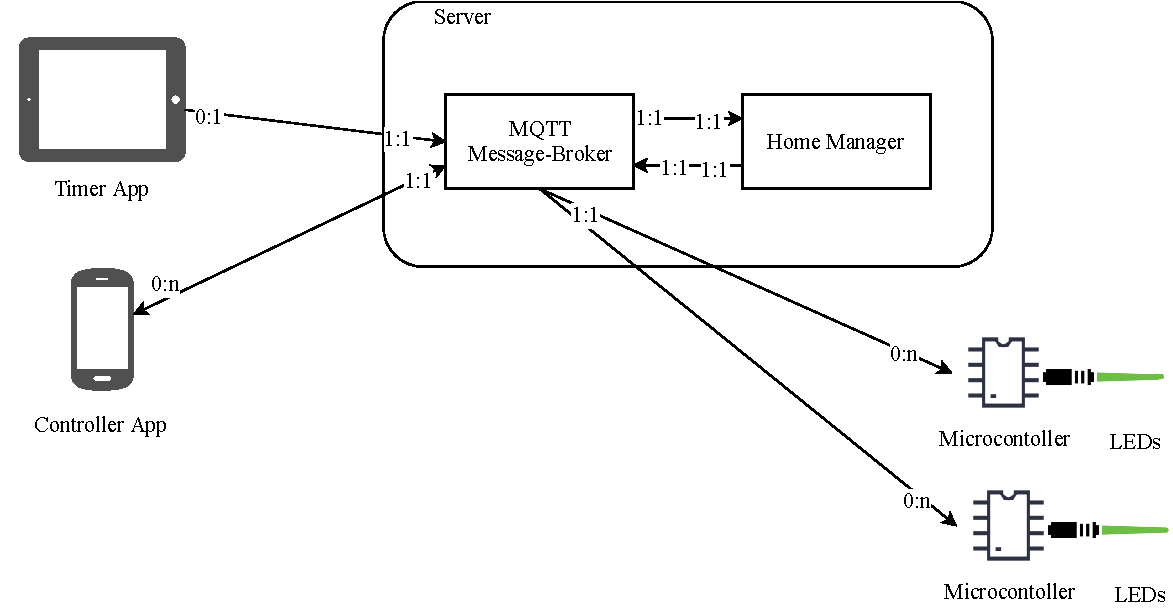
\includegraphics[width=\linewidth]{../images/architecture}
	\caption[Architektur der Smart-Home Infrastruktur]{Architektur der Smart-Home Infrastruktur}
	\label{fig:architecture}
\end{figure}


\section{Funktionale Anforderungen}

Die Infrastruktur der SmartHome-Anwendung soll dazu in der Lage sein, die folgenden Anwendungsfälle zu unterstützen:
\begin{itemize}
	\item Es ist möglich, sich mit jedem möglichen Gerät im Netzwerk (im Speziellen dem WLAN-Netzwerk) anzumelden und bestimmten Topics zuzuhören und Nachrichten zu diesen zu senden. So kann später auch eine Anwendung für Windows-PCs oder eine Webanwendung entwickelt werden. Diese Arbeit beschäftigt sich nur mit der Implementierung zweier Android-Apps als Frontend.
	\item Durch die Anmeldung der empfangenden Geräte, wie in dieser Arbeit die verwendeten LED-Lichterkette, kann prinzipiell jedes angemeldete Gerät angesteuert werden. Ein anderer denkbarer Ansatz wäre beispielsweise die Ansteuerung von Jalousinen über die beschriebene Infrastruktur.
	\item Die Server-Komponente auf dem Raspberry Pi übernimmt dabei besondere Aufgaben, die entweder zentral verwaltet werden müssen, wie bpsw. Timer-Funktionalität (siehe \ref{home_manager}), oder die nicht auf den Mikrocontrollern realisiert werden können (siehe \ref{impl_mikrocontroller}).
\end{itemize}

\section{Nicht-funktionale Anforderungen}

Neben den funktionalen Anforderungen müssen einige nicht-funktionale Anforderungen erfüllt werden, um die Erstellung und Weiterentwicklung der Lösung zu gewährleisten. Dazu zählen insbesondere
\begin{itemize}
	\item die Erstellung eines sauberen Programmcodes, sodass auch spätere Entwickler weiterhin am Projekt arbeiten können.
	\item die Performanz der Lösung, damit diese frustfrei verwendet werden kann.
	\item die Absturzsicherheit der verschiedenen Programme, sodass keine manuellen Neustarts oder dergleichen getätigt werden müssen. 
	\item die Übersichtlichkeit der Apps, damit der Nutzer diese möglichst intuitiv bedienen kann.
	\item die Skalierbarkeit, sodass spätere Komponenten möglichst einfach hinzugefügt werden können.
\end{itemize}




			\chapter{Implementierung}



\section{App zur LED-Steuerung} \label{impl_steuer_app}

\subsection{Aufbau der Anwendung}
Die Anwendung soll auf der Startseite die Ansicht eines Colorpickers darstellen, sodass sofort nach Start der App eine Farbe ausgewählt werden kann. Diese Farbe wird sofort ohne Bestätigung an die ausgewählte LED Leiste gesendet. \\
Über einen Navigation-Drawer vom linken Bildschrim sind neben dem bereits ausgewählten Reiter \textit{Colorpicker} noch die Reiter \textit{Effects}, \textit{State} und \textit{Settings} auswählbar. Diese haben folgende Funktionalitäten:
\begin{description}
	\item[Effects] Zeigt alle möglichen Effekte, die der Home Manager momentan umsetzen kann. Durch einen Klick auf die entsprechende Schaltfläche wird der Effekt auf der ausgewählten LED Leiste wiedergegeben.
	\item[State] Diese Ansicht zeigt die Zustände (Farbe, Effekt) der LEDs, die sich momentan im Netzwerk befinden. Diese Liste wird vom Home Manager geliefert.
	\item[Settings] Hier werden die nötigen Einstellungen getroffen. Momentan zählen hierzu die Adresse und der Port, unter der der Message-Broker erreichbar ist. Zusätzlich werden hier die Topics der einzelnen LEDs festgelegt, damit diese in anderen Teilen einfach ausgewählt werden können.
\end{description}

\subsection{Funktionale Anforderungen}

Die Funktionen wurden teilweise schon im vorherigen Abschnitt erläutert. Im Allgemeinen kann die App als eine grafische Oberfläche zur Erstellung \& dem Versenden der verschiedenen JSON-Nachrichten gesehen werden. Die App stellt einen grafischen Colorpicker dar, wovon sich der Benutzer eine Farbe aussuchen kann. Sobald diese ausgewählt wurde, wird ein Listener aufgerufen, der den Farbcode des Colorpickers in RGB umwandelt und diese Informationen über entsprechende Objekte in ein JSON-Objekt umwandelt. Dieses wird mit dem vorher ausgewählten Topic, das über einen Button repräsentiert wird, auf das Netzwerk geschrieben, wodurch der Rest der Infrastruktur die LED zum Leuchten bringt. \\
Die JSON-Dokumente werden dabei von einer selbst erstellten Klasse \textit{JsonBuilder} erstellt. Diese ist nach dem Builder-Pattern aufgebaut, sodass möglich einfach ein neues JSON-Dokument erstellt und in neue Komponenten eingepflegt werden kann.\\
Beim Reiter \textit{Effects} werden entsprechend andere Teile des JSON-Dokuments eingefügt, sodass der Mikrocontroller diese versteht und die Effekte wie Regenbogen darstellt. \\
Im Reiter \textit{State} befindet sich eine Liste aller in der App hinterlegten LEDs. Hier wird immer ein Paar aus dem Namen der LED, welcher in den anderen Komponenten angezeigt wird, und dem Topic der LED hinterlegt. Das Hinzufügen wird über einen Floating Action Button vorgenommen, der einen Dialog öffnet, in dem die Informationen eingetragen werden. Einzelne LEDs können mit einem langen Klicken des Elements einfach gelöscht werden. \\
Die letzte Seite \textit{Settings} beinhaltet die Verbindungsparameter, des Message Brokers im Netzwerk. Hier wird die IP und der Port des Servers eingetragen, welche in den Shared Preferences abgelegt und im Rest der Anwendung verwendet werden.


\section{Implementierung der Timer-App} \label{impl_timer_app}
Neben der Steuerungs-App für die LED-Leisten wurde eine weitere Android Applikation entwickelt, welche abhängig vom Fortschritt eines Timers eine LED-Leiste als Fortschrittsanzeige ansteuert.\\
Für eine Verwendung auf einem Tablet in einer Küche ist es wichtig, mehrere parallele Timer zu erstellen und diese auf einer Seite gleichzeitig laufen zu lassen. Bei der Entwicklung sollte berücksichtigt werden, dass auch Benutzer ohne Smart Home Infrastrukutur die App verwenden können. Hierfür wird zwischen den beiden Flavors \gf{default} und \gf{mqtt} unterschieden. Die MQTT Flavor enthält alle Funktionalitäten der normalen Applikation und zusätzlich Funktionalitäten zur Integration in das Smart Home System.

\subsection{Funktionale Anforderungen}
Die Applikation soll folgende Anforderungen zuverlässig erfüllen:
\begin{itemize}
	\item Mehrere Timer erstellen und zeitgleich ablaufen zu lassen. Dabei sollen mehrere Timer gleichzeitig sichtbar sein.
	\item Beim Ablauf eines Timers soll visuell und akustisch auf den Ablauf hingewiesen werden.
	\item Auch beim Schließen der Applikation sollen die Timer im Hintergrund weiterlaufen.
\end{itemize}
Zusätzlich sollen bei Verbindung mit einem MQTT-Broker folgende Funktionalitäten umgesetzt werden (nur in der Flavor \gf{mqtt}):
\begin{itemize}
	\item Konfigurieren eines MQTT Servers und eine automatische Verbindung mit dem Server bei App-Start
	\item Die Auswahl eines Timers in der App überträgt automatisch den aktuellen Fortschritt (Prozentual die abgelaufene Zeit zu der restlichen Zeit) an eine LED Kette. Hierbei wird die LED-Leiste in zwei Teile unterteilt, welche in verschiedenen Farben angezeigt werden
	\item Beim Ablauf eines Timers signalisiert die LED Leiste, dass ein Timer abgelaufen ist. Dies wird durch eine blinkende LED-Leiste repräsentiert.
\end{itemize}

\subsection{Aufbau der Anwendung}
Wie in Diagramm \ref{fig:timerapparchitektur} gezeigt, besteht die App aus zwei Teilen. Der auch im Hintergrund laufende Service beinhaltet die Logik des sekündlichen Herunterzählens und verwaltet alle Timer. Die Benutzeroberfläche zeigt diese Werte in einem GridView an, wobei der Benutzer auch über die UI die Timer ändern kann. Das eigentliche Ändern der Objekte wird allerdings wieder von dem Service gemacht.
\begin{figure}
	\centering
	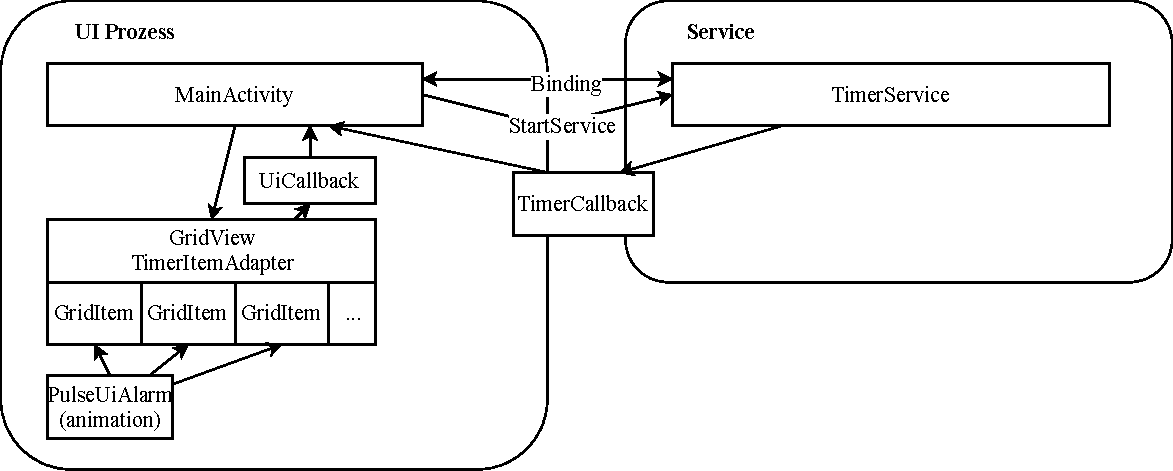
\includegraphics[width=\linewidth]{../images/timer_app_architektur}
	\caption[Timer App Überblick]{Timer App Überblicksarchitektur}
	\label{fig:timerapparchitektur}
\end{figure}


\section{Mikrocontroller} \label{impl_mikrocontroller}
Das in C geschriebene Programm für die einzelnen LED Steuereinheiten wurde als \gf{thin client} umgesetzt. Das heißt, dass nur möglichst einfache Funktionen auf dem Mikrocontroller ausgeführt werden und die komplette Logik auf die steuernden Clienten (siehe \ref{impl_steuer_app} und \ref{impl_timer_app}) und dem Manager (siehe \ref{home_manager}) verschoben werden.\\
Mit der Arduino PubSubClient MQTT Library hört der Mikrocontroller ständig, ob eine neue Nachricht auf ein relevantes Topic angekommen ist. Wenn eine Nachricht ankommt, wird diese durch die \gf{ArduinoJson} Library geparsed und die Werte ausgelesen. Anschließend werden die verarbeiteten Werte mittels der Adafruit Neopixel Library auf die digitalen LEDs geschrieben. Sobald alle LEDs neu beschrieben wurden, hört der Mikrocontroller wieder auf neue Nachrichten vom MQTT Broker.

%\section{Home Manager Modul} \label{home_manager}
%Das Home Manager Modul ist eine Serverkomponente, die Funktionen ausübt, die nicht vom Clienten direkt ausgeführt werden können oder einen erheblichen Mehraufwand der Clientapplikationen bedeuten würde. Der Manager hat mehrere Funktionen, die sich in folgende drei Klassen einteilen lassen.
%\begin{description}
%	\item [Ereignisabhängige Funktionen] können vom Manager verwaltet und ausgeführt werden. Das einfachste Beispiel sind LEDs, die zu einer bestimmten Zeit angeschaltet werden sollen. Hierbei soll ein Clientgerät nur den Auftrag geben, die LEDs anzumachen aber keine Nachricht direkt an die LEDs senden. Hierdurch ist es möglich ein Handy Nachts im Flugzeugmodus zu haben und trotzdem zu einer bestimmten Uhrzeit von langsam angehenden LEDs geweckt zu werden.\\
%	Andere Ereignisse könnten von internen Triggern ausgeführt werden oder von Diensten wie If-This-Then-That gesteuert werden. Diese Funktionalität soll ich Umfang der Projektarbeit sein.
%	\item [Statusüberblick Funktionen] verhelfen allen Geräten synchron mit dem aktuellen Zustand der LEDs zu bleiben. Der Manager notiert bei jeder Änderung von einem Ausgabegerät den neuen Zustand und speichert diesen in einer Datenbank. Wenn sich ein neues Gerät anmeldet, kann dieses die Informationen zu anderen Geräten vom Manager erfragen.
%\end{description}
			\chapter{Ablauf des Projektes}

\section{Projektorganisation}
Das Projekt wurde von Patrick Sudhaus und Alexander Hatzold verwirklicht. Aufgrund der geringen Dienstwege wurde keine besondere Form der Projektorganisation gewählt. Die Anforderungen wurden initial festgelegt und dann gemeinsam umgesetzt.

\section{Technische Schwierigkeiten \& deren Lösung}

\subsection{Verwendung einer Microcontroller MQTT Library}
Ein Problem, welches bei der Implementierung des Mikrocontroller Programms aufgetreten ist, war die Entscheidung die Adafuit\_MQTT\_Library zu verwenden. Diese Library beschränkt MQTT Nachrichten auf eine Länge von 128 Bytes pro Nachricht. Die JSON-Nachrichten überschreiten manchmal diese Größe, sodass nicht die gesamte Nachricht übermittelt wird und somit nicht verarbeitbar ist. Da auch Anpassung der Library nicht erfolgreich war musste eine andere Library verwendet werden. Die Library \textit{pubsubclient}\footnote{\url{https://pubsubclient.knolleary.net/}} hat eine viel höhere Längenbeschränkung, wodurch sie für den use-case geeignet ist. Ein Problem beim PubSub Client sind die fehlenden QOS Level eins und zwei bei ausgehenden Nachrichten. Das heißt, dass es möglich ist, dass Nachrichten unbemerkt nicht ankommen können (siehe \ref{introMQTT}). Da die Mikrocontroller nur Nachrichten empfangen ist dies aktuell nicht relevant.

\subsection{Fehlende Nebenläufigkeit auf den Microcontrollern}
Da die Microcontroller basierend auf ESP8266 keine Nebenläufigkeit unterstützen, musste sich für bestimmte Funktionalitäten eine andere Lösung überlegt werden, um gleichzeitig einen Befehl auszuführen (z.B. LED Lauflicht Effekte) und gleichzeitig andere Befehle zu erhalten (z.B. neue Nachrichten vom MQTT Broker empfangen) und zu starten. Die Parallelität wurde deswegen teilweise auf die Serverkomponente \textit{Home Manager} (siehte Abschnitt \ref{home_manager}) ausgelagert, sodass alle gewünschten Funktionen realisierbar sind.
			
			\chapter{Fazit \& Auswertung?}

ALEX?
			
			
			
			\clearpage
			
		\pagenumbering{roman}
			
			\bibliographystyle{plaindin}
			\bibliography{../bibliography/bib_smarthome}
			
			\glsaddall
			
			%\newpage
			%\printglossary[type=\acronymtype, toctitle=Abkürzungen, title=Abkürzungen]
			%\newpage
			%\printglossary[title=Glossar, toctitle=Glossar, style=altlist]

			%\layout

			\appendix

			%\input{../appendix/appendix}

			%\input{../chapters/Anhang/bilder}

			%\input{../chapters/Anhang/dokumente}
			

\end{document}